% !TEX encoding = UTF-8 Unicode
% !TEX spellcheck = en_US
\documentclass{svproc}
\usepackage{paralist}
\usepackage{amsmath}
\usepackage{amssymb}
\newcommand{\bm}[1]{\boldsymbol{#1}}

% Latex-Makros für häufig verwendete Formelzeichen
\newcommand{\ortvek}[4]{{ }_{(#1)}{\boldsymbol{#2}}^{#3}_{#4} }
\newcommand{\vek}[3]{\boldsymbol{#1}^{#2}_{#3}}
\newcommand{\rotmat}[2]{{{ }^{#1}\boldsymbol{R}}_{#2}}
\newcommand{\rotmato}[2]{{{ }^{#1}\boldsymbol{\overline{R}}}_{#2}}
\newcommand{\transp}[0]{{\mathrm{T}}}
\newcommand{\ks}[1]{{\mathcal{F}}_{#1}}

% Für Deutsche Umlaute
%\usepackage{ngerman}
\usepackage[utf8]{inputenc}

% Für Bilder
\usepackage{graphicx}
\usepackage{color}
\graphicspath{{./figures/}}

% to typeset URLs, URIs, and DOIs
\usepackage{url}
\def\UrlFont{\rmfamily}

\begin{document}
    
\mainmatter              % start of a contribution
%
\title{Exploiting Dynamics Parameter Linearity for Design Optimization in Combined Structural and Dimensional Robot Synthesis}
%
\titlerunning{Parameter Linearity in Design Optimization}  % abbreviated title (for running head)
%                                     also used for the TOC unless
%                                     \toctitle is used
%
\author{Moritz Schappler \and Svenja Tappe \and Tobias Ortmaier}
%
\authorrunning{Schappler et al.} % abbreviated author list (for running head)
%
%%%% list of authors for the TOC (use if author list has to be modified)
%\tocauthor{Moritz Schappler, Svenja Tappe, and Tobias Ortmaier}
%
\institute{Institute for Mechatronic Systems, Leibniz University Hannover, Germany,\\
    \email{moritz.schappler@imes.uni-hannover.de}}

\maketitle              % typeset the title of the contribution


%ABSTRACT
\begin{abstract}
In the design optimization of robot manipulators regarding drive train and link geometries the dynamics equations have to be evaluated repeatedly.
The method proposed in this paper reduce the computational effort in the dynamics evaluations by using the property of parameter linearity of the dynamics equations.
The combined structural and dimensional synthesis of robot manipulators is adapted in a set of hierarchical optimization loops to exploit this dynamics property.
By this means a reduction of computation time for the inverse dynamics in the synthesis of up to factor five can be expected.
\end{abstract}

%KEYWORDS
\begin{keywords}
Robot Design Optimization, Dynamics Regressor Form, Combined Structural and Dimensional Synthesis
\end{keywords}

\section{Introduction and State of the Art}
\label{sec:Intro}

% Was ist Entwurfsoptimierung? Einordnung

% Entwurfsoptimierung wird eingesetzt, um vom Menschen erdachte Maschinen so zu parametrieren, dass sie gestellte Anforderungen bestmöglich erfüllen.
Design optimization formalizes the process of designing technical systems done by engineers and allows to find values for the design parameters with optimization algorithms based on given objectives and constraints.
% Die Parametrierung kann sich am Beispiel von Robotern auf Kinematik-Parameter wie die Längen der Segmente beziehen, auf die Auslegung der Strukturteile und auf die Auswahl und Auslegung des Antriebsstrangs.
In the case of robotic systems the design parameters can be the lengths of the robot links, the shape of the links or the selection of the drive train components motor and gearbox.
The parameters can be deduced from the robot structure which consists of the type and principal alignment of the robots joints and is determined in the \emph{structural synthesis} of the robot.

% Abgrenzung Auslegung der Kinematikparameter und Entwurfsoptimierung
In this paper we distinguish between the optimization of parameters with influence on the kinematics and the optimization of parameters only influencing other characteristics of the robot such as the dynamics.
%Ansätze für Optimierung der Kinematikparameter
%Mehrkriterielle Optimierung von kinematischen Zielgrößen wie Arbeitsraum und Robotergröße [CeccarelliLan2004] oder zusätzlich Berücksichtigung statischer Zielgröße wie eines Steifigkeitsmodells für serielle und parallele Roboter [CarboneOttCec2007] oder dynamischer Zielgrößen, wie der über die Trajektorie verbrauchten Energie [RamirezKotOrt2017]
The optimization of kinematic parameters is referred to as \emph{dimensional synthesis} and can be implemented as multi-criterial optimization of kinematic criteria like workspace and robot size \cite{CeccarelliLan2004}, static criteria like stiffness \cite{CarboneOttCec2007} or dynamics-based criteria like energy consumption \cite{RamirezKotOrt2017}.
%Die Entwurfsoptimierung bezüglich kinematischer Parameter kann auch gemeinsam mit die Dynamik beeinflussenden Parametern wie eines parametrischen CAD-Modells  [TarkianLunÖl2008,ZhouBai2015] oder der Antriebsstrangauslegung [ShillerSun1991] erfolgen
A combined optimization of parameters influencing kinematics and dynamics can be performed by using parametric CAD models \cite{TarkianLunOel2008,ZhouBai2015} or by combined optimization of link and drive train properties \cite{ShillerSun1991}.

% Überblick über Entwurfsoptimierung für Roboter hinsichtlich Antriebsstrang und Segmenten

%Auslegung des Antriebsstrangs:
% Grundprinzip ist eine gegebene Roboterstruktur mit definierten Kinematikparameter, dessen Antriebe an eine gegebene Trajektorie oder Punkt-zu-Punkt-Bewegung angepasst werden \cite{ChedmailGau1990}
For the \emph{optimal selection of drive train components} separate from the kinematics parameters, these can be regarded as given. % full trajectory or start and end points of the
% Zielfunktion der Optimierung ist eine kurze Zykluszeit \cite{TarkianPerOelFen2011}, Masse der Antriebe \cite{ChedmailGau1990,PetterssonOel2009,ZhouBaiHan2011}, Lebensdauer der Getriebe \cite{PetterssonAndKru2005}, monetäre Kosten \cite{PetterssonAndKru2005}
Common objective functions are the drive train mass \cite{ChedmailGau1990,PetterssonOel2009,ZhouBaiHan2011}, the trajectory cycle time \cite{TarkianPerOelFen2011}, the predicted life time of the gears \cite{PetterssonAndKru2005} or monetary costs \cite{PetterssonAndKru2005}.
%Nebenbedingungen sind die Bemessungsmomente und Drehzahl von Motor und Getriebe [ChedmailGau1990,PetterssonOel2009,ZhouBaiHan2011], 
Constraints contain at least the speed and torque limits of the components \cite {ChedmailGau1990,PetterssonOel2009,ZhouBaiHan2011}.

% Mögliche zusätzliche Erweiterungen der Simulation des Systems sind eine zusätzliche Dynamik aus einem thermischen Motormodell [ChedmailGau1990] oder die Berechnung der Vorwärtsdynamik des geregelten Systems mit Betrachtung des Regelfehlers und der elektrischen Motordynamik [Padilla-GarciaCruRod2015], anstelle der reinen Betrachtung der inversen Dynamik mit Vernachlässigung regelungstechnischer Effekte.
It is usually sufficient to regard the inverse rigid body dynamics without considering electric, thermal or control effects.
The extension of the robot simulation within the optimization has been done for thermal dynamics in \cite{ChedmailGau1990} and for electrical and controller dynamics in \cite{Padilla-GarciaCruRod2015}.


% Auslegung der Struktur
The \emph{optimization of the parameters of the robot links} like the engineering design can be achieved with parametrized CAD-models prepared by a designer for the specific robot \cite{TarkianPerOelFen2011,ZhouBai2015} or by using geometric primitives \cite{RamirezKotOrt2017} for approximations. %  if creating CAD models is not possible in the case of a multiplicity of robot structures in a combined structural and dimensional synthesis
% Bei Optimierung der Strukturparameter kann ebenfalls deren Masse als Zielfunktion verwendet werden [TarkianPerOelFen2011]
The most straight-forward objective function for the link optimization consists of the masses of the links which also correlates with energy consumption and joint torques.
Constraints can be implemented by performing stress analysis on the links CAD model using FEM programs like CATIA \cite{TarkianPerOelFen2011} or Ansys \cite{ZhouBai2015}.
The load on the links and on the motors can be calculated using multibody programs like Modelica/Dymola \cite{TarkianPerOelFen2011}, ADAMS \cite{ZhouBaiHan2011} or by using optimized code from symbolic calculations \cite{ChedmailGau1990} which reduces the computation \cite{KhalilDom2002}.

% Die Ansätze können weiterhin darin unterschieden werden, ob die Trajektorie im Zeitverlauf Teil der Optimierung ist [PetterssonAndKru2005], oder ob diese als konstant gegeben ist [TarkianPerOelFen2011,ZhouBaiHan2011,Padilla-GarciaCruRod2015].
The approaches presented until here can be separated into cases, where the trajectory does not change within the design optimization \cite{TarkianPerOelFen2011,ZhouBaiHan2011,Padilla-GarciaCruRod2015} and cases, where the trajectory is part of the optimization and only start and end pose of the end effector are given \cite{PetterssonAndKru2005,PetterssonOel2009,TarkianPerOelFen2011}.
% Bei einer zusätzlichen Optimierung der Segmentlängen ist aufgrund der Neuberechnung der inversen Kinematik auch die Neuberechnung der Trajektorie erforderlich [TarkianLunÖl2008,ZhouBai2015]
The trajectory changes within the optimization, if it is part of the objective function or if the kinematic parameters change in the optimization \cite{TarkianLunOel2008,ZhouBai2015}, since the trajectory is usually given in task space and has to be transferred to joint space via the inverse kinematics.


% Der Optimierungsalgorithmus zur Berücksichtigung der diskreten Entwurfsvariablen sind genetische Algorithmen [TarkianPerOelFen2011,Padilla-GarciaCruRod2015], Particle Swarm Optimierung [RamirezKotOrt2017] oder Complex-Algorithmus mit Modifikationen bezüglich der Rundung und Interpolation in der Auswahltabelle  [PetterssonAndKru2005] [ZhouBaiHan2011] oder die Interpolation der Auswahltabelle und Überführung in ein kontinuierliches Problem [ChedmailGau1990]
For the discrete problem of selecting components of given gearbox and motor databases genetic algorithms \cite{TarkianPerOelFen2011,Padilla-GarciaCruRod2015}, particle swarm optimization \cite{RamirezKotOrt2017} and the complex-algorithm with modifications regarding rounding and interpolation of the selection database \cite{PetterssonAndKru2005,ZhouBaiHan2011} can be used.
% Je nach Art der Annahmen über die Antriebe und Segmente ist ein rekursives Vorgehen von distalen zu proximalen Gelenken möglich [ChedmailGau1990].
Depending on the assumptions on the placement of actuators, a recursive joint-wise approach from distal to proximal joints is possible and simplifies the optimization \cite{ChedmailGau1990}.
% ...zur Berücksichtigung  der diskreten Entwurfsvariablen Complex, PSO, GA
% ...sind Gradientenbasierte Verfahren [], Simplex [TarkianPerOelFen2011]

% ...Eine Bewertung von computergenerierten Strukturen ist damit ebenfalls möglich



% Kurzfassung des Beitrags des Papers
The overview of the state of the art shows, that the field of design optimization for robot manipulators has made great progress in the last decade.
One central element in the design optimization is the calculation of the robot dynamics, which should be implemented as efficient as possible.
% Alle bisherigen Arbeiten zur Entwurfsoptimierung vernachlässigen die Eigenschaft der Parameterlinearität der Dynamik-Gleichungen, die hauptsächlich aus dem Bereich Parameteridentifikation bekannt ist.
One method to improve the computation time spent on inverse dynamics calculations is to use the linearity of the dynamics equation with respect to the dynamics parameters.
Regrouping the parameters to a minimal form allows to improve the performance even further \cite{KhalilDom2002}, which is a key to the success of parameter identification experiments.
To the best knowledge of the authors, the properties of the dynamics regressor form are not fully exploited by the design optimization community.
%[ChedmailGau1990] nennt zwar die Nutzung der parameterlinearen Form zur Berechnung der Dynamik und geht auf die Anpassung der Parameter ein, die Ausnutzung der Parameterlinearität in der Entwurfsoptimierung wird aber nicht erwähnt. Da auch keine der folgenden Arbeiten darauf eingehen, wird dieser Aspekt in diesem Paper hervorgehoben.

With the regressor form, it is possible to split the dynamics calculation into two steps: The calculation of the regressor matrix and the  multiplication of the regressor matrix with the dynamics parameter vector.
Under certain assumptions the dynamics calculation in the design optimization process can then be performed with the second step.
The first step can be done outside the optimization loop, since the regressor matrix is dependent on the kinematics of the robot, which stays the same in the inner loop.

The contributions of this paper are
\begin{compactitem}
    % Präsentation eines Ansatzes zur schnelleren Berechnung der inversen Dynamik für die Entwurfsoptimierung von Mehrkörpersystemen, insbesondere von Manipulatoren
    \item the presentation of an approach for a faster calculation of the inverse dynamics in the design optimization of robot manipulators,
    % Vorstellung eines Konzepts zur kombinierten Struktur- und Maßsynthese von seriellen und parallelen Robotern, Darstellung der Annahmen für die schnellere Berechnung
    \item a concept for the combined structural and dimensional synthesis of serial and parallel robots exploiting this dynamics formulation,
    % Beispielhafte Rechnungen zum Aufzeigen der Vorteile durch das Verfahren
    \item examples on the possible reduction of the computation time.
\end{compactitem}

The remainder of the paper is structured as follows:
% * Vorstellung des Konzepts der kombinierten Struktur- und Maßsynthese und Herleitung des Bedarfs einer effizienten Entwurfsoptimierung
The combined structural and dimensional synthesis is briefly presented as a motivation and field of application for the proposed method in Sec.\,\ref{sec:DimSynth}.
% * Zeigen der Eigenschaften der verwendeten Dynamikmodellierung 
The properties of the dynamics model are summed up in Sec.\,\ref{sec:DynMdl}.
% * Einsatz dieser Dynamikmodellierung in der Entwurfsoptimierung
% * Überschlägige Rechnung zum Potential der Verbesserung
The possible improvement of the design optimization is explained in Sec.\,\ref{sec:DesOptImprove} with an estimate on the computational costs in Sec.\,\ref{sec:Example}.
% * Zusammenfassung

\section{Combined Structural and Dimensional Synthesis}
\label{sec:DimSynth}

%[RamirezKotOrt2015]
% Idee der kombinierten Struktur- und Maßsynthese: Für eine gegebene Roboteraufgabe mit Freiheitsgraden und Trajektorie und Last werden alle geeigneten seriellen und parallelen Strukturen ermittelt und davon die bestgeeignesten ausgewählt.
The synthesis of robot manipulators can be divided in two phases.
The first phase is finding the number, kind and alignment of joints in the \emph{structural synthesis}.
To obtain a result with quantifiable performance, the dimensioning of the parameters regarding actuation, gears, link lengths and link geometry have to be defined in the \emph{dimensional synthesis} as a second phase.
Usually the two phases are performed separately and the choice of a structure is done by the designer.
Combining both phases means to perform the dimensional synthesis for all possible kinematic structures for a task with given degrees of freedom and trajectory as  sketched in Fig.\,\ref{fig:structdimsynth} for the whole process.
This allows a comparison of all $N_{\mathrm{S}}$ different structures with optimized dimensions for the given task and to select the robot structure that is suited best \cite{RamirezKotOrt2015,RamirezKotOrt2017}.


\begin{figure}[tb]
	\input{./figures/comb_struct_dim_synth.pdf_tex}
	\caption{Overview of the procedure for combined structural and dimensional synthesis. The degrees of freedom (DoF) of the task are given in the $\alpha\mathrm{T}\beta\mathrm{R}$-notation for the numbers of translational DoF  $\alpha$ and of rotational DoF $\beta$.}
	\label{fig:structdimsynth}
\end{figure} 

% Dadurch wird der Vergleich einer Vielzahl von Strukturen notwendig. Z.B. 10 für 2T1R, 35 für 3T1R, 326 für 3T3R serielle Strukturen.
% Für Parallele Strukturen ergeben sich ebenfalls eine Vielzahl an Kombinationen, wie z.B. von Gogu mit Hilfe der evolutionären Morphologie ermittelt [Gogu].

%Dadurch, dass mehrere verschachtelte Schleifen durchlaufen werden ist die Rechenzeit relativ hoch. Besonders der Rechenaufwand für die innere Schleife ist entscheidend für die Gesamtlaufzeit des Algorithmus
Despite the existence of methods to reduce the number of kinematic structures from the structural synthesis to a minimum \cite{RamirezKotOrt2015}, the computational effort in the dimensional synthesis is still high.
For serial chain robots e.\,g. with the assumption of non-redundancy and only parallel and orthogonal joints there exist 10 possible configurations for planar motions (2T1R), 35 for Schönflies motions (3T1R, ``SCARA'') and 326 for general motions (3T3R) \cite{RamirezKotOrt2015,RamirezKotOrt2017}.
An even higher number of parallel robot structures exists due to the possibility of overconstraint, non-symmetry and selection of joint actuation, which are listed in \cite{Gogu2008} and its following parts.

%Nennung der Schleifen: Über alle Roboter, Über alle Kinematikparameter, Antriebs- und Segmentauslegung basierend auf inverser Dynamik zu allen Zeitschritten der Trajektorie
% Blockschaltbild mit ungefährem Gesamtablauf
The high computational effort required for the combined synthesis is caused by the multiplicity of optimization loops, namely from outside to inside
\begin{compactenum}
\item a loop over all $N_{\mathrm{S}}$ possible robot structures,
\item the optimization of the kinematic parameters $\bm{\varrho}$ (length of links),
\item the design optimization of the drive train and the link geometry affecting the dynamics parameters $\bm{\delta}$ and requiring the dynamics calculation in 
\item a loop over all $N_\mathrm{T}$ sample points of the given trajectory.
\end{compactenum}

The loops 2 to 4 are summarized in Fig.\,\ref{fig:dimsynth_dyn_std}, which depicts the nested optimization loops in a block diagram that corresponds to the dimensional synthesis block of Fig.\,\ref{fig:structdimsynth}.
There, the first loop is highlighted by the depicted stacked blocks.
The time dependent quantities end effector pose $\bm{x}(t)$, joint coordinates $\bm{q}(t)$ and joint torque $\bm{\tau}(t)$ are assumed to contain the full time series and the needed time derivatives over all $N_\mathrm{T}$ samples of the trajectory.

\begin{figure}[tb]
    \input{./figures/dim_synth_dynamics_standard.pdf_tex}
    \caption{Overview of the placement of inverse dynamics calculation in the nested optimization loops of dimensional synthesis.}
    \label{fig:dimsynth_dyn_std}
\end{figure} 

% Für die Berechnung Dynamischer Leistungsmerkmale wie Gesamtmasse oder Energie (basierend auf den Gelenkmomenten) ist die Berechnung der inversen Dynamik notwendig.
When using only kinematic performance measures like workspace size or dexterity for the dimensional synthesis, the dynamics do not have to be evaluated and the third loop is not necessary, which simplifies the optimization.
On the other hand when using dynamics performance measures or when the decision for a robot structure also incorporates the possibilities of the actuation, all loops have to be taken into account.

% Damit der Vergleich zwischen stark verschiedenen Strukturen mit möglichst wenigen Kennzahlen möglich ist:
% Annahme für die Maßsynthese: Trajektorie bleibt gleich
% Ansonsten müsste beim Vergleich der Strukturen verschiedene Kennzahlen wie Arbeitsraum, Fußabdruck, Energieverbrauch und zusätzlich die Verfahrdauer der Trajektorie einkriteriell gewichtet oder mehrkriteriell z.B. mittels Pareto-Front vergleichen werden.
%Durch die Vorgabe der Trajektorie wird die Komplexität reduziert und die im Folgenden dargestellte Methode wäre nicht möglich.
To reduce the computational effort, the trajectory $\bm{x}(t)$ is regarded as given and not as part of the optimization.
This does not allow to use the point-to-point cycle time as a performance measure.
On the upside, the comparison of different structures like serial and parallel robots is reduced in complexity and it allows to use the method proposed in the latter part of the paper.
The demand for the reduction of complexity can be justified by the fact, that serial and parallel robots have completely different characteristics regarding their performance criteria like workspace, footprint, accuracy, stiffness, energy or dynamics.
These criteria have to be traded off against each other in a single-objective or multi-objective optimization.
Comparing the dynamics or energy for different structures each with different time-series of the trajectory would again raise the question of how to weight these performance measures against each other.


\section{Properties of the Dynamics Model}
\label{sec:DynMdl}

The inverse dynamics equations are used in the design optimization of robot links and drive trains as can be seen in Fig.\,\ref{fig:dimsynth_dyn_std}.
Its purpose is to calculate the torque on the motor and the forces and moments on the links to evaluate if the considered configuration is feasible.
Additionally, the properties of motor, gearbox and link affect the dynamics parameters and therefore the result of the equations.
Since this paper focuses on the rigid body dynamics, other effects such as friction are neglected and the quantities of the drive train like motor torque, motor inertia and gear ratio are assumed to be included in the joint space equations and are omitted in the following.
This section defines the dynamics model in a nomenclature suitable to show the improvement of the design optimization in the next section and corresponds to textbook-knowledge \cite{KhalilDom2002}.

To investigate the influence of the kinematic and dynamics parameters, the parameters are written explicitly in the equations.
The kinematics parameters $\bm{\varrho}$ contain the parameters from the joint transformations according to the modified Denavit-Hartenberg notation and are e.\,g. the lengths of the links.
%
The dynamics parameters are defined in three representations:
\begin{compactitem}
\item The barycentric dynamics parameters of each link $i$ consist of the link mass $m_i$, the three coordinates $\ortvek{i}{r}{}{C_i}$ of the links center of mass $C_i$ (CoM)  expressed in the respective link frame and six entries of the symmetric inertia tensor $\ortvek{i}{I}{(C_i)}{}$ w.\,r.\,t the links CoM. 
\item The inertial parameters are related to the origin $O_i$ of the link frame and contain the links mass $m_i$, the first moment $m_i \ortvek{i}{r}{}{C_i}$ and the second moment $\ortvek{i}{I}{(O_i)}{}=\ortvek{i}{I}{(C_i)}{}+m_i\bm{S}^\transp(\ortvek{i}{r}{}{C_i})\bm{S}(\ortvek{i}{r}{}{C_i})$ which can be calculated with the Huygens-Steiner theorem using the skew-operator $\bm{S}$.
The $10$ inertial parameters for link $i$ are stacked in $\bm{\delta}_i$ and the $10N$ parameters for all $N$ links are stacked in the vector $\bm{\delta}$.
\item The base inertial parameters can be obtained by combining the inertial parameters with set of rules to the linear relation $\bm{\beta}=\bm{K}(\bm{\varrho})\bm{\delta}$.
\end{compactitem}
%

%[KhalilDom2002]
% Dynamikmodell allgemein in verallgemeinerten Koordinaten, Grundlage für Antriebsauslegung (Modell mit Antrieb?)
% Keine Formulierung der Dynamik auf Motorseite oder mit Getriebeübersetzung. Hinweis, dass die Umrechnung weiterhin so geschieht wie bisher, und dass die Motorträgheit mit der Getriebeübersetzung auf die Abtriebseite umgerechnet werden kann
The joint torques $\bm{\tau}$ of a serial-chain robot manipulator are calculated with the inverse dynamics model
%
\begin{align}
\bm{\tau} 
&= 
\bm{M}(\bm{q},\bm{\varrho},\bm{\delta}) \ddot{\bm{q}}
+ \bm{c}(\bm{q},\dot{\bm{q}},\bm{\varrho},\bm{\delta})
+ \bm{g}(\bm{q},\bm{\varrho},\bm{\delta}) \label{equ:invdyn_normal} 
= \bm{\tau}(\bm{q},\dot{\bm{q}},\ddot{\bm{q}},\bm{\varrho},\bm{\delta})\\
&=
\bm{\Phi}_{\bm{\tau}}(\bm{q},\dot{\bm{q}},\ddot{\bm{q}},\bm{\varrho}) \bm{\delta}
\label{equ:invdyn_reg}
\end{align}
%
in the joint coordinates $\bm{q}$.
It contains the effects of inertia $\bm{M}$, centrifugal and Coriolis forces $\bm{c}$ and gravity $\bm{g}$ and is linear in the inertial parameters $\bm{\delta}$ with the regressor matrix $\bm{\Phi}_{\bm{\tau}}$.

By deriving the dynamics with the Newton-Euler-Algorithm, it is also possible to express the internal forces $\bm{f}_i$ and moments $\bm{m}_i$ in the joints $i$ in the parameter linear form
\begin{equation}
\bm{w}_i = 
\begin{pmatrix} \bm{f}_i^\transp & \bm{m}_i^\transp\end{pmatrix}^\transp
=
\bm{\Phi}_{\bm{w}_i}(\bm{q},\dot{\bm{q}},\ddot{\bm{q}},\bm{\varrho}) \bm{\delta}.
\label{equ:joint_wrench}
\end{equation}

% Eigenschaft der Regressorform: Obere rechte Dreiecksform; die Gelenkmomente der letzten Achsen hängen nur von den letzten Dynamikparametern ab, die Gelenkmomente der ersten Achse hängen von allen Parametern ab. Dünne Besetztheit der Regressormatrix kann genutzt werden.
The regressor matrices $\bm{\Phi}_{\bm{\tau}}$ and 
$\bm{\Phi}_{\bm{w}}$
have the upper triangular form
\begin{equation}
\bm{\Phi}=
\begin{pmatrix} \bm{\Phi}_{1} \\ \bm{\Phi}_{2} \\ \vdots \\ \bm{\Phi}_{N}
\end{pmatrix}
=
\begin{pmatrix} \bm{\Phi}_{1,\bm{\delta}_1} & \bm{\Phi}_{1,\bm{\delta}_2} & \dots & \bm{\Phi}_{1,\bm{\delta}_N} \\
\bm{0} & \bm{\Phi}_{2,\bm{\delta}_2} & \dots & \bm{\Phi}_{2,\bm{\delta}_N} \\
\vdots & \ddots & \ddots & \vdots \\
\bm{0} & \bm{0} & \bm{0} & \bm{\Phi}_{N,\bm{\delta}_N}
\end{pmatrix},
\label{equ:regressor_triangular}
\end{equation}
where the influence of the inertial parameters of link $j$ on joint $i$ is marked by $\bm{\Phi}_{i,\bm{\delta}_j}$.
%
This shows the property of serial kinematic chains, that the inertial parameters of links proximal to the robot base have no influence on distal joints.

% Parameterlineare Form der Dynamik
% Prinzip der Parametergruppierung: Zusammenfassung von Parametern vom Endeffektor zur Basis
% Zeigen anhand der Regressormatrix der Inertialparameter mit Formel. Beschreibung der rekursiven Kombinationsvorschriften und daraus resultierender ähnlicher Form für den Minimalparameter-Regressor.
The dynamics equation (\ref{equ:invdyn_normal}-\ref{equ:invdyn_reg}) can also be expressed with the base\footnote{``base'' refers to the minimal set of parameters in the mathematical sense.} inertial parameters $\bm{\beta}$.
These parameters are obtained with a recursive combination of inertial parameters with the same effect on the joint torque.
Parameters without effect are removed from the parameter vector.
Due to the recursive scheme from the end-effector link to the base link, the regressor matrix with respect to the base inertial parameters has a similar upper triangular form as in (\ref{equ:regressor_triangular}).
Exploiting this known structure allows further reduction of the computational load.

% Für Segmentauslegung: Gelenkmomente sind allein nicht ausreichend. Bei Verwendung der Schnittkräfte in den Gelenken vor und nach dem Segment ist ebenfalls eine parameterlineare Darstellung möglich, allerdings sind durch Parameterzusammenfassung keine oder wesentlich weniger Vereinfachungen möglich als bei alleiniger Betrachtung der Gelenkmomente.
The joint torque equation (\ref{equ:invdyn_normal}) can be used for design optimization of the drive train.
For the optimization of link parameters, the full internal forces and moments from (\ref{equ:joint_wrench}) should be used.
Equation (\ref{equ:joint_wrench}) can not be expressed with the base parameters, since all inertial parameters affect the internal forces and no parameter reduction is possible.
In the following, the regressor with respect to the inertial parameters $\bm{\delta}$ will be used in this paper for the sake of simplicity.
The base parameter regressor should however be used in the implementation wherever possible, since it is more efficient.

The equations and remarks above refer to serial robots.
The dynamics of parallel robots can also be expressed in a regressor form, since it can be derived by projection of the legs and platform dynamics into the task space.
Grouping the parameters to a set of base inertial parameters again allows the reduction of the complexity.
The scheme described in the following section can therefore also be applied to parallel robots.

\newpage

\section{Improve the Efficiency of Design Optimizing}
\label{sec:DesOptImprove}

With the assumptions from Sec.\,\ref{sec:DimSynth} of an unchangeable task space trajectory and a separate optimization of kinematic and dynamics parameters, the presented properties of the dynamics equations from Sec.\,\ref{sec:DynMdl} can be used to accelerate the evaluation of the dynamics equations in the dimensional synthesis.

Since the inverse kinematics can be calculated in the second loop (over the kinematics parameters $\bm{\varrho}$) and the dynamics equations are evaluated in a third loop (of the drive train optimization updating $\bm{\delta}$), the joint space trajectory $\bm{q}(t)$ can be regarded as given in the third loop.
Then, as depicted in Fig.\,\ref{fig:dimsynth_dyn_plin}, the property (\ref{equ:invdyn_reg}) of linearity of the dynamics equation can be used to divide it into the calculation of the regressor matrices $\bm{\Phi}(t)$ in the second loop and the multiplication of the regressor with the dynamics parameter vector  $\bm{\delta}$ in the third loop.
The regressor $\bm{\Phi}_{\bm{w}}$ for the full internal forces $\bm{w}$ from (\ref{equ:joint_wrench}) can be used in the same manner and is omitted in Fig.\,\ref{fig:dimsynth_dyn_plin} for clarity.

% Formel: Optimierungsproblem
% Formel: Ausklammern des Regressors aus einer Operation
% Blockschaltbild Optimierung ohne Ausnutzung der Parameterlinearen Form
% Blockschaltbild Optimierung mit Ausnutzung
\begin{figure}[tb]
    \input{./figures/dim_synth_dynamics_plin.pdf_tex}
    \caption{Sketch of the improved calculation of dynamics in the nestested optimization loops of dimensional synthesis. The numbers of the loops are referenced in the text.}
    \label{fig:dimsynth_dyn_plin}
\end{figure} 



%Rekapitulation der Annahme: Ist nicht möglich, wenn die Kartesische Trajektorie verändert wird und indirekt Zielfunktion der Optimierung ist [TarkianÖlFenPet2009,PetterssonOel2009,TarkianPerOelFen2011] oder Nebenbedingung [PetterssonAndKru2005] ist oder wenn die Kinematischen Längen Teil der Optimierung sind [TarkianLunÖl2008,ZhouBai2015]
% ...oder die Nebenbedingungen beeinflusst.

\section{Exemplary Calculations}
\label{sec:Example}

% Aussage: Bei Verwendung des Ausklammerns der Dynamikgleichungen kann man ...% der Rechenzeit sparen.
Using the linearity of dynamics parameters as described above reduces the computational cost of evaluating the dynamics equations down to the multiplication of the regressor matrix with the parameter vector.
%The effort to calculate the matrix is neglected assuming a sufficient number of iterations in the third loop.
Table\,\ref{tab:computation} gives an estimate on the computational cost for the dynamics of three different serial chain robots: A 4-DoF SCARA robot, a 6-DoF industrial robot arm manipulator and the 7-DoF DLR/Kuka Light Weight Robot (LWR).
The upper part of Table\,\ref{tab:computation} shows the properties of the robots kinematic and dynamics parameters (rows ``A''-``D'').
The lower part summarizes the computational cost of the dynamics using direct calculation from the right-hand side of (\ref{equ:invdyn_normal}) in one case (row ``G'') and solely the regressor multiplication of (\ref{equ:invdyn_reg}) in the second case (row ``H'').
Both calculations are implemented using the base parameter regressor form and all possible optimizations to ensure a fair comparison.
%The data is given for the regressor matrix $\bm{\Phi}_{\bm{\tau}}$, referred to the base parameter vector $\bm{\beta}$, since this is the most efficient form.
The dynamics equations are implemented as \textsc{Matlab} functions, which are compiled for faster execution.
% and are able to run on real-time controllers like PLC or Simulink-based testbeds.
The code is generated by the computer algebra system \textsc{Maple} using generalized joint coordinates, kinematics based on homogenous transformation matrices, a formulation of the energy of the multy body system w.r.t. the inertial dynamics parameters, the Lagrangian equations of the second kind and a base parameter regrouping algorithm, see \cite{KhalilDom2002}.
Code optimization is done by \textsc{Maple}, also exploiting the sparsity of the triangular form (\ref{equ:regressor_triangular}) of the regressor, which can be recognized from the ratios of zeros given in table row ``E''.
%Further details are omitted at this place due to space limitations and the focus of the paper on the dimensional synthesis.
The number of operations in the table contains the unweighted sum of the number of additions, multiplications and assignments of temporary variables.

Since the calculation using a given regressor matrix is much simpler, the computational effort can be decreased in theory over 80\,\%, as highlighted in table row ``I''.
However, some aspects reduce the savings in the practical implementation:
\begin{compactitem} 
\item Saving the $\mathrm{dim}(\bm{q}) \times \mathrm{dim}(\bm{\beta})$ regressor matrices for all $N_\mathrm{T}$ trajectory samples leads to additional overhead in the memory access,
\item the regressor matrix has to be computed beforehand, which will pay off more, if the dynamics are evaluated very often in the inner optimization loop.
\end{compactitem}  

% Tabelle mit EE-FG, Anzahl Gelenke, Anzahl Kinematikparameter, Dimension Regressor, Anzahl Nullen, Operationen Dynamik aus Regressor, Operationen Matrix-Multiplikation.
% Für Drei Roboter: LBR, Kuka 6FG, SCARA


\begin{table}[tb]
    \caption{Overview of the parameter properties and the computational effort for inverse dynamics calculation for three serial robot examples.}
    \label{tab:computation}
    \centering
    \setlength\tabcolsep{3pt}
    \small
    \begin{tabular}[t]{|l||l|c|c|c|} 
        \hline
         & Robot & SCARA & Ind. Robot & LWR \\
        \hline
        A & $\mathrm{dim}(\bm{q})$: number (\#) of joint DoF  & 4 & 6 & 7 \\
        B & $\mathrm{dim}(\bm{\varrho})$: \# of kinematic parameters & 2 & 6 & 3 \\
        C & $\mathrm{dim}(\bm{\delta})$: \# of inertial parameters & 40 & 60 & 70 \\
        D & $\mathrm{dim}(\bm{\beta})$: \# of base inertial parameters  & 10 & 38 & 45 \\ %\footnotemark
        E & ratio of zeros in the $\bm{\beta}$-regressor $\bm{\Phi}_{\bm{\tau}}$ & 19/40 & 87/228  & 124/315 \\
        &  &  = 48\,\% &  = 38\,\% &  = 39\,\% \\
        \hline
        F & \# of operations for one regressor evaluation & 327 & 1796 & 3003 \\
        \hline
        G & \# of operations for one dynamics evaluation & 328 & 2078 & 3385 \\
        H & \# of operations for regressor multiplication & 42 & 282 & 382 \\
        I & decrease using regressor multiplication & 87\,\% & 86\,\% & 89\,\% \\
        \hline
    \end{tabular}
    \vspace{-0.5cm}
\end{table}
%\footnotetext{Assuming floor mounting with fixed direction of gravity instead of the chosen general direction of gravity allows further simplifications with the parameter reduction.}

The reduction of computation time is evaluated at the example of one loop of the dimensional synthesis (block ``2'' in Fig.\,\ref{fig:dimsynth_dyn_std} and Fig.\,\ref{fig:dimsynth_dyn_plin}) for the three serial chain robots of Table\,\ref{tab:computation}.
The computation time on the vertical axis is plotted for different numbers of dynamics parameters iterations in the design optimization of the actuators(block ``3'' in Fig.\,\ref{fig:dimsynth_dyn_plin}).
% TODO: actuation, only joint torque
The time for the calculation of the joint torque regressor matrix (\ref{equ:regressor_triangular}) is added to the time needed for the multiplication in  (\ref{equ:invdyn_reg}) of all dynamics parameter iterations and is marked as ``RegMult''.
The direct calculation of the inverse dynamics of (\ref{equ:invdyn_normal}) or of block ``3''/``4'' of Fig.\,\ref{fig:dimsynth_dyn_std} is marked as ``InvDyn''.

The left part of Fig.\,\ref{fig:timing_evaluation} shows the absolute computation time of the inverse dynamics for a complete joint trajectory with $N_{\mathrm{T}}{=}1000$ samples.
%
The ``RegMult''-method (dashed lines in Fig.\,\ref{fig:timing_evaluation}, left) already outperforms the ``InvDyn''-method at five or more iterations of the dynamics parameters.
This can be explained by the low computational cost of the regressor matrix, listed in row ``F'' of Table\,\ref{tab:computation}, which is approximately as high as one dynamics evaluation.
Since the sparsity of the regressor matrix is exploited by the symbolic optimizations in the ``InvDyn''-method, it was also implemented for the ``RegMult''-method by storing only the non-zero elements of the matrix as one row vector per time step.
%To ensure a fair comparison, the sparsity of the regressor matrix was also exploited for the matrix-vector-multiplication, by storing only the non-zero elements of the matrix as one row vector per time step.

The influence of the length of the trajectory is investigated with the right part of Fig.\,\ref{fig:timing_evaluation} at the example of the 7-DoF LWR.
The ratios of the computation times for ``RegMult'' and ``InvDyn'' are compared for different lengths of the trajectory.
The ``RegMult''-method is faster, if the line is below 100\,\%.
%, which is the case for more than five dynamics iterations.
The method benefits from a higher number of trajectory samples, which converges to a time reduction of 70\,\% for $N_{\mathrm{T}}>100$ and more than 50 dynamics iterations.

\begin{figure}[tb]
    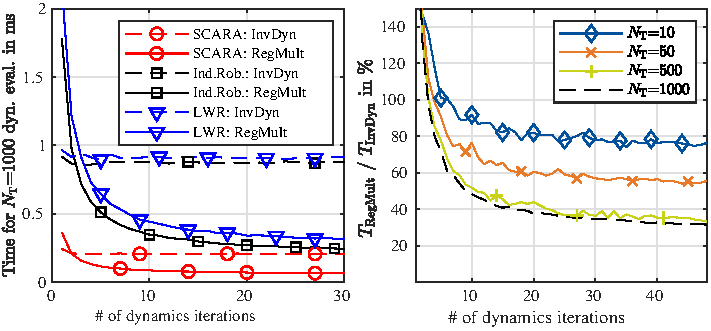
\includegraphics{./figures/dyn_timing_eval.pdf}
    \caption{Left: Comparison of the computation time for inverse dynamics for three robots and two methods. Right: Ratio of the computation times for different trajectory lengths.}
    \label{fig:timing_evaluation}
\end{figure} 


\section{Conclusions}
\label{sec:Conclusion}


% Vorstellung des Verfahrens zur Ausnutzung ...
% Ausblick: Anwendung des Verfahrens zum Vergleich von seriellen und parallelen Robotern in der kombinierten Struktur- und Maßsynthese.

This paper presents an optimization scheme to select robot manipulators for a given task in a combined structural and dimensional synthesis.
The optimization required to find the best suitable manipulator consists of nested loops of selecting different structures, optimizing kinematic parameters and optimizing dynamics parameters via design optimization of drive train and link properties.
The loops are arranged in a way to improve the efficiency of the whole process by exploiting the parameter linearity of the dynamics equations.
\newpage
\section*{Acknowledgements}

The financial support from the Deutsche Forschungsgemeinschaft (DFG) under grant number OR 196/33-1 is gracefully acknowledged.

% BIBLIOGRAPHY
\bibliographystyle{spmpsci_unsrt}
\bibliography{dimsynth_minpar_ref}

\end{document}
